\section{VisPerf}

Since Perf outputs a lot of data, we propose VisPerf to easily visualize and compare the data captured. The VisPerf pipeline can be seen as three stages: capture, processing and visualization.

In the capture stage, the person recognition stream application is executed using the two mapping policies discussed before and profiled with Perf. We configured Perf to sample 997 times each second the application is running. The raw data from Perf is converted to a CSV file for posterior analysis.

In the second stage, the CSV files are processed and merged. In summary, the processing stage groups captures made within the same second, extract the three top functions in the stack executing on the CPU, and also label the threads. This stage generates a JSON file that is used in the visualization stage. The JSON file contains the structured data of each experiment and also the details of the hardware where experiments were executed, allowing quick data reading on the VisPerf dashboard. In addition, generating a single JSON file with all experiments makes it simple to share data for analysis between researchers.

After these two stages end, VisPerf dashboard can be accessed to analyze captured data. In Section~\ref{section:visualization-interaction}, we discuss the visualizations and interactions we propose to VisPerf dashboard.


\subsection{Visualizations and Interactions} \label{section:visualization-interaction}

The first step inside VisPerf is to upload the JSON file generated in the processing stage. VisPerf reads this file and generates the plots. We used D3\footnote{\url{https://d3js.org}} library to create the visualizations as it is very customizable and has many features to allow users to interact with the plots. Since the JSON file file may contains many experiments, we allow the user to select two experiments they want to compare.

VisPerf visualization is divided into three sections. The first section, showed in Figure~\ref{figure:visperf-section-1}, is named ``Comparing experiments''. This section compares specific events captured while executing the two experiments selected. As shown in Figure~\ref{figure:visperf-section-1}, the user can select the event to be compared and the plot. For this section, there are two plots available: the parallel coordinates and another plot with a grid representing the CPUs available in the processor where experiments were executed.

\begin{figure}[ht]
    \centering
    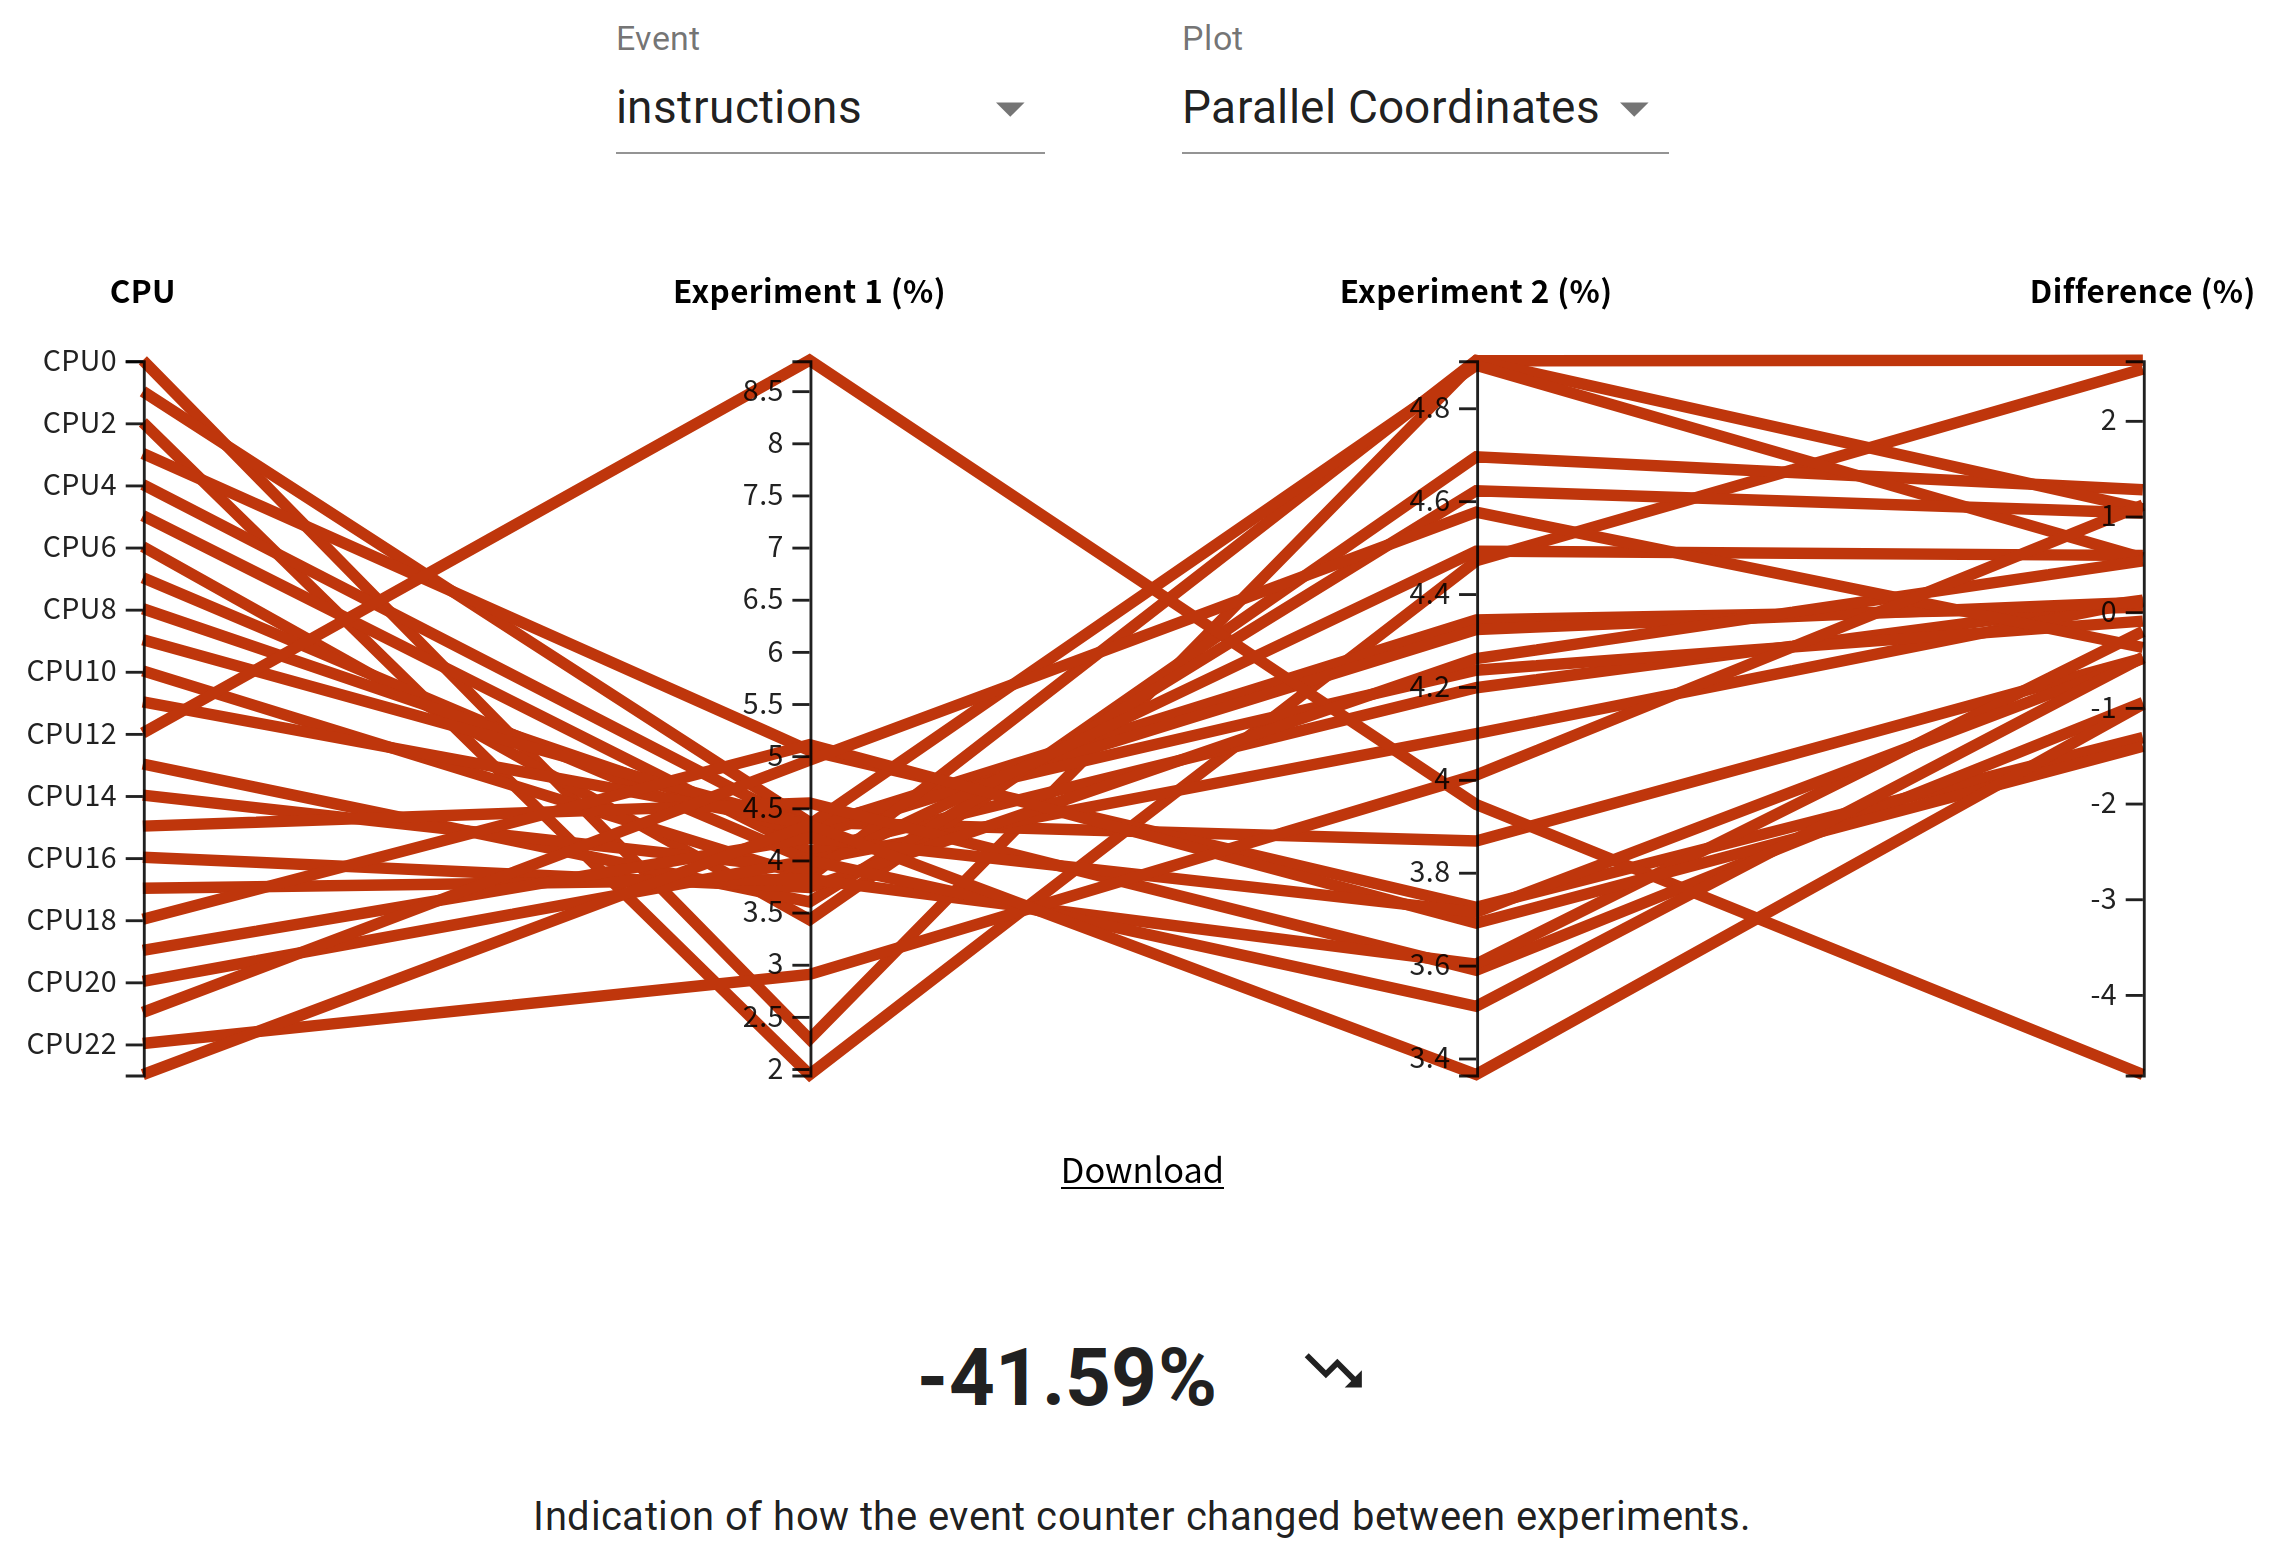
\includegraphics[width=1.0\columnwidth]{../pictures/visperf-section-1.png}
    \caption{VisPerf section ``Comparing experiments''.}
    \label{figure:visperf-section-1}
\end{figure}

The first section in VisPerf also shows a summary of how the event selected changed between the experiments. As shown in Figure~\ref{figure:visperf-section-1}, the second experiment required 41.59\% fewer instructions to finish execution. Another important metric this plot shows is that the second experiment had a better balance between the CPUs. CPU 12, for example, executed $\approx$ 9\% of the instructions, while in experiment two most of the CPUs executed $\approx$ 5\% of the instructions. The last column in the parallel coordinates plot shows the absolute difference between CPUs.

As the CPU number increases, the parallel coordinate plot starts to be a bit confusing because of the high number of lines. However, when hovering a specific line, this line is highlighted and the opacity of other lines decreased. Another feature that is present in all plots is the download button. Here, the plots are downloaded in SVG format, which can be converted to any other format by the user.

\begin{figure}[ht]
    \centering
    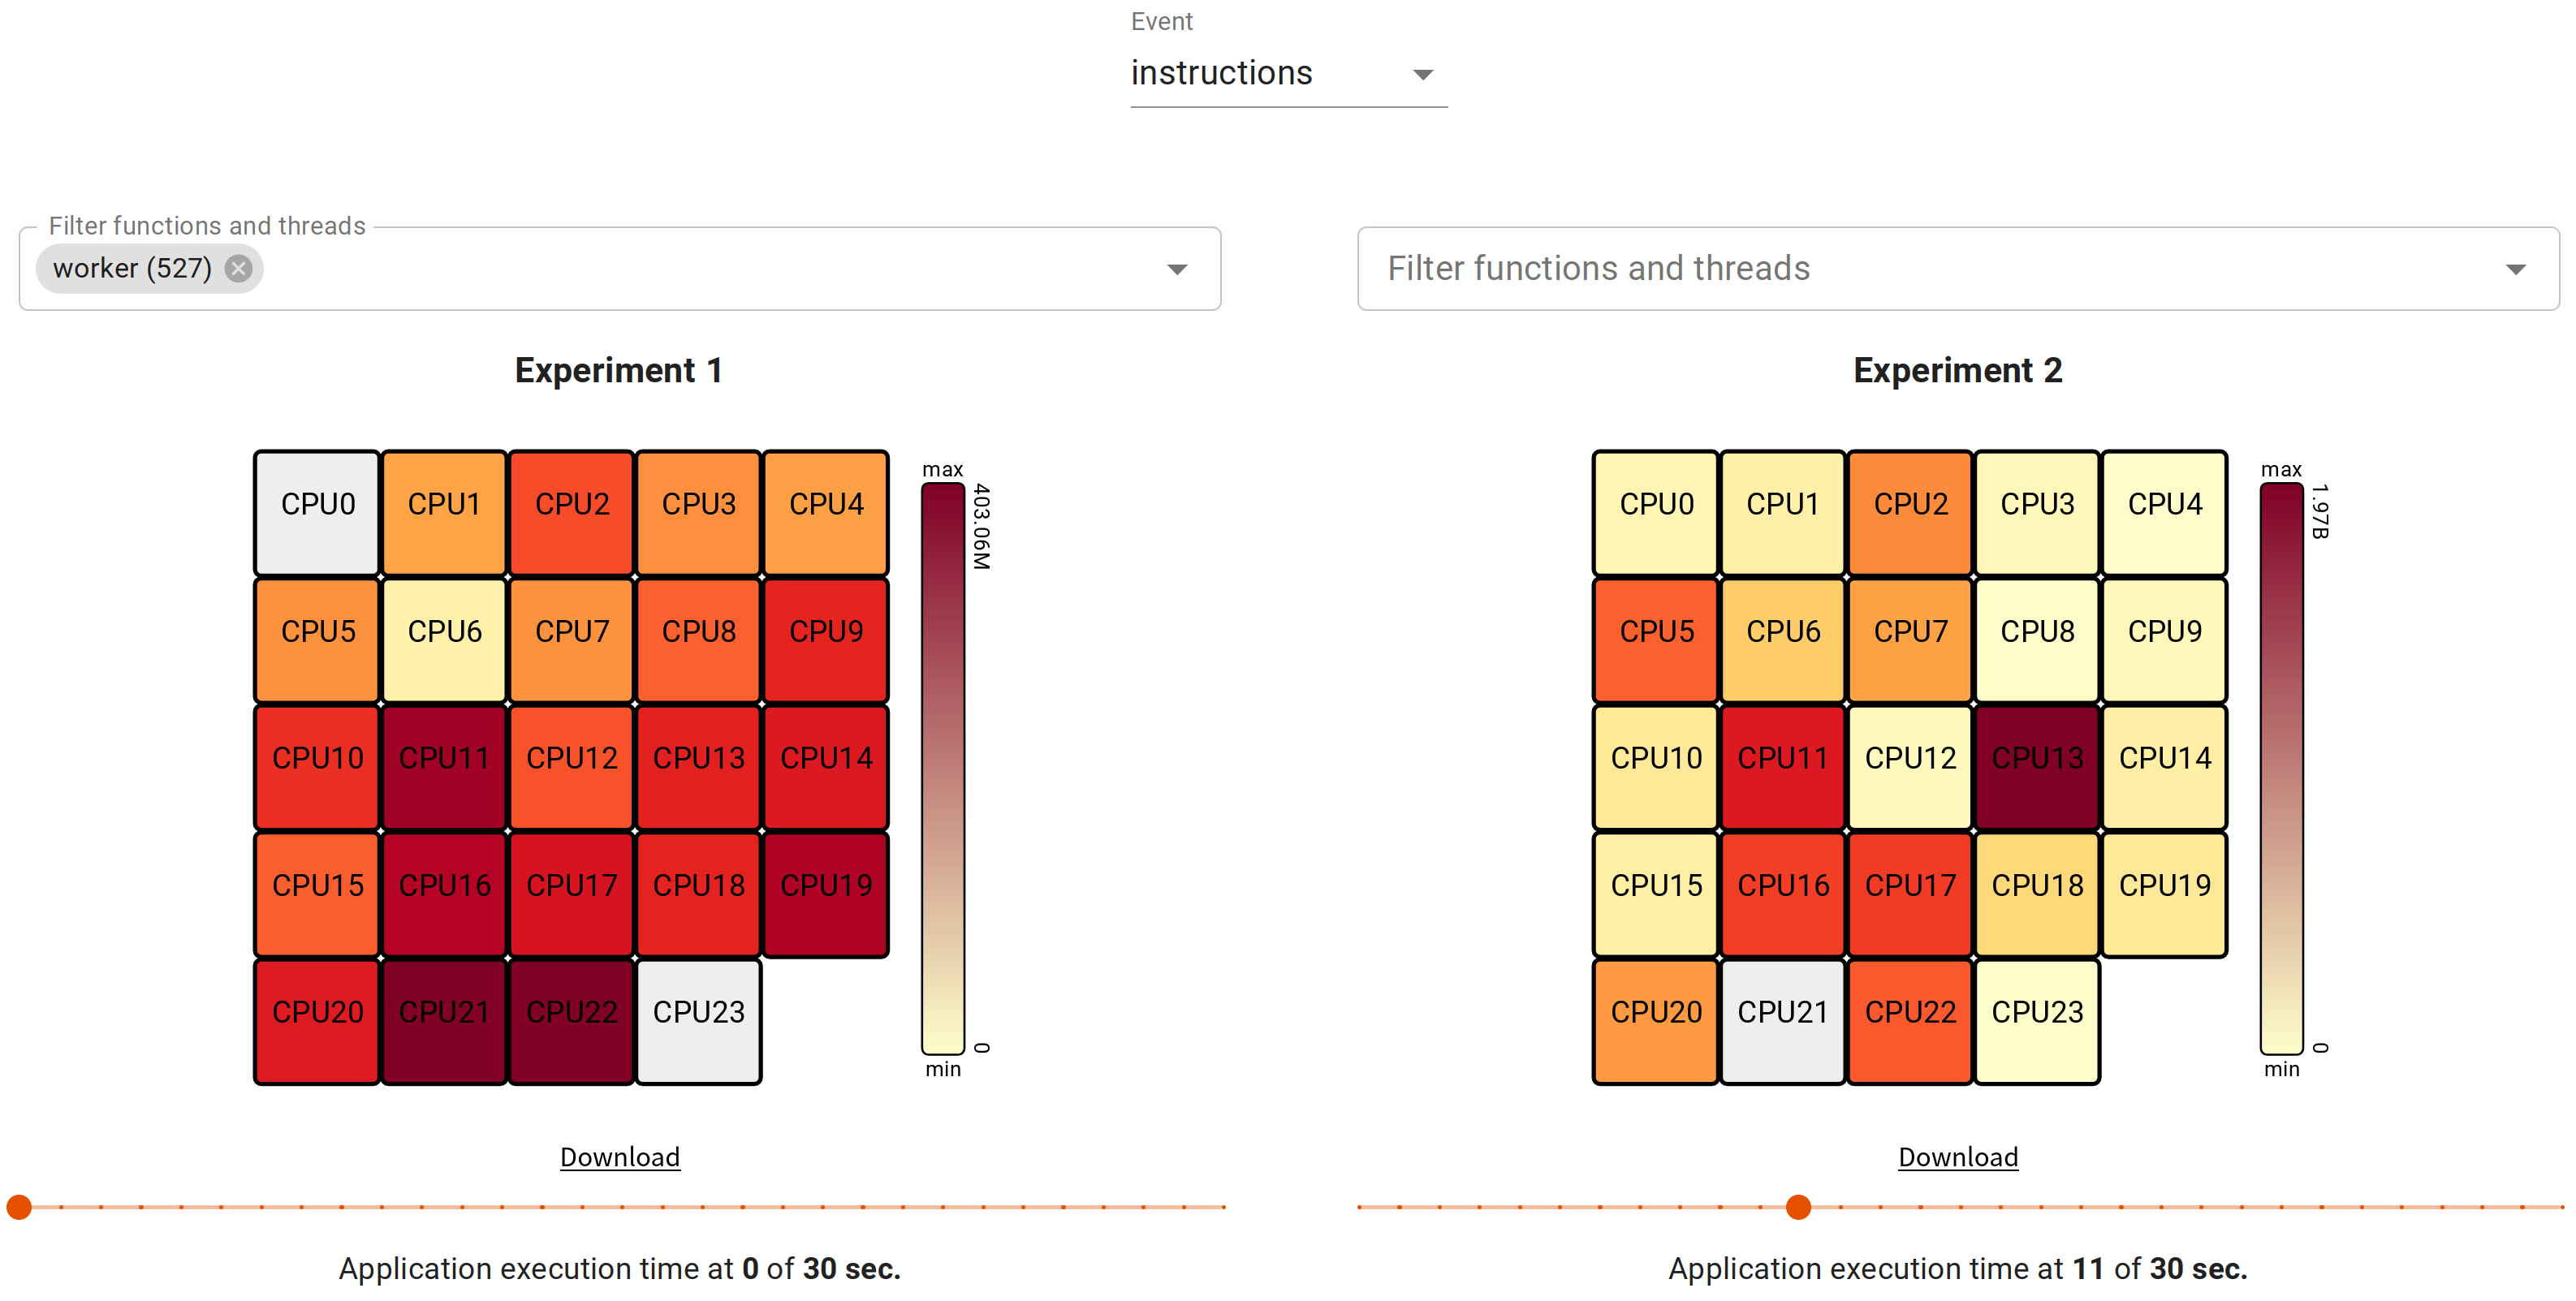
\includegraphics[width=1.0\columnwidth]{../pictures/visperf-section-2.png}
    \caption{VisPerf section ``Comparing experiments over execution time''.}
    \label{figure:visperf-section-2}
\end{figure}

The second section, named ``Comparing experiments over execution time'' and shown in Figure~\ref{figure:visperf-section-2}, allows the user to explore the performance of specific functions or threads executed on the application. Since Perf only captures the thread id, we modified the source code of the application to inform the function being executed on the specific threads. Therefore, thread ids that are not present at the program output are named as ``Other threads''. In addition, in the second section, the user can view the metrics of the PMUs at specific points of the application execution. Navigating in the experiment one, shown in Figure~\ref{figure:visperf-section-2}, we can see that CPUs 0 and 23 were not used. While in experiment two, all CPUs are used, and at some points, some threads migrated of CPU while running the person recognition application. This behavior is correct because experiment one is using a fixed mapping policy, proposed by FastFlow, and experiment two the default operating system mapping policy.

The last section of VisPerf has metrics that use the events captured by Perf. For now, we only have one metric: IPC (Instructions Per Cycle). This metric indicates the average number of instructions executed at each CPU cycle. This section has two view dimensions: over time or by CPU. Over time visualization shows how IPC vary over the application execution time and by CPU visualization shows the IPC variation between the CPUs used to run the application.

\begin{figure}[ht]
    \centering
    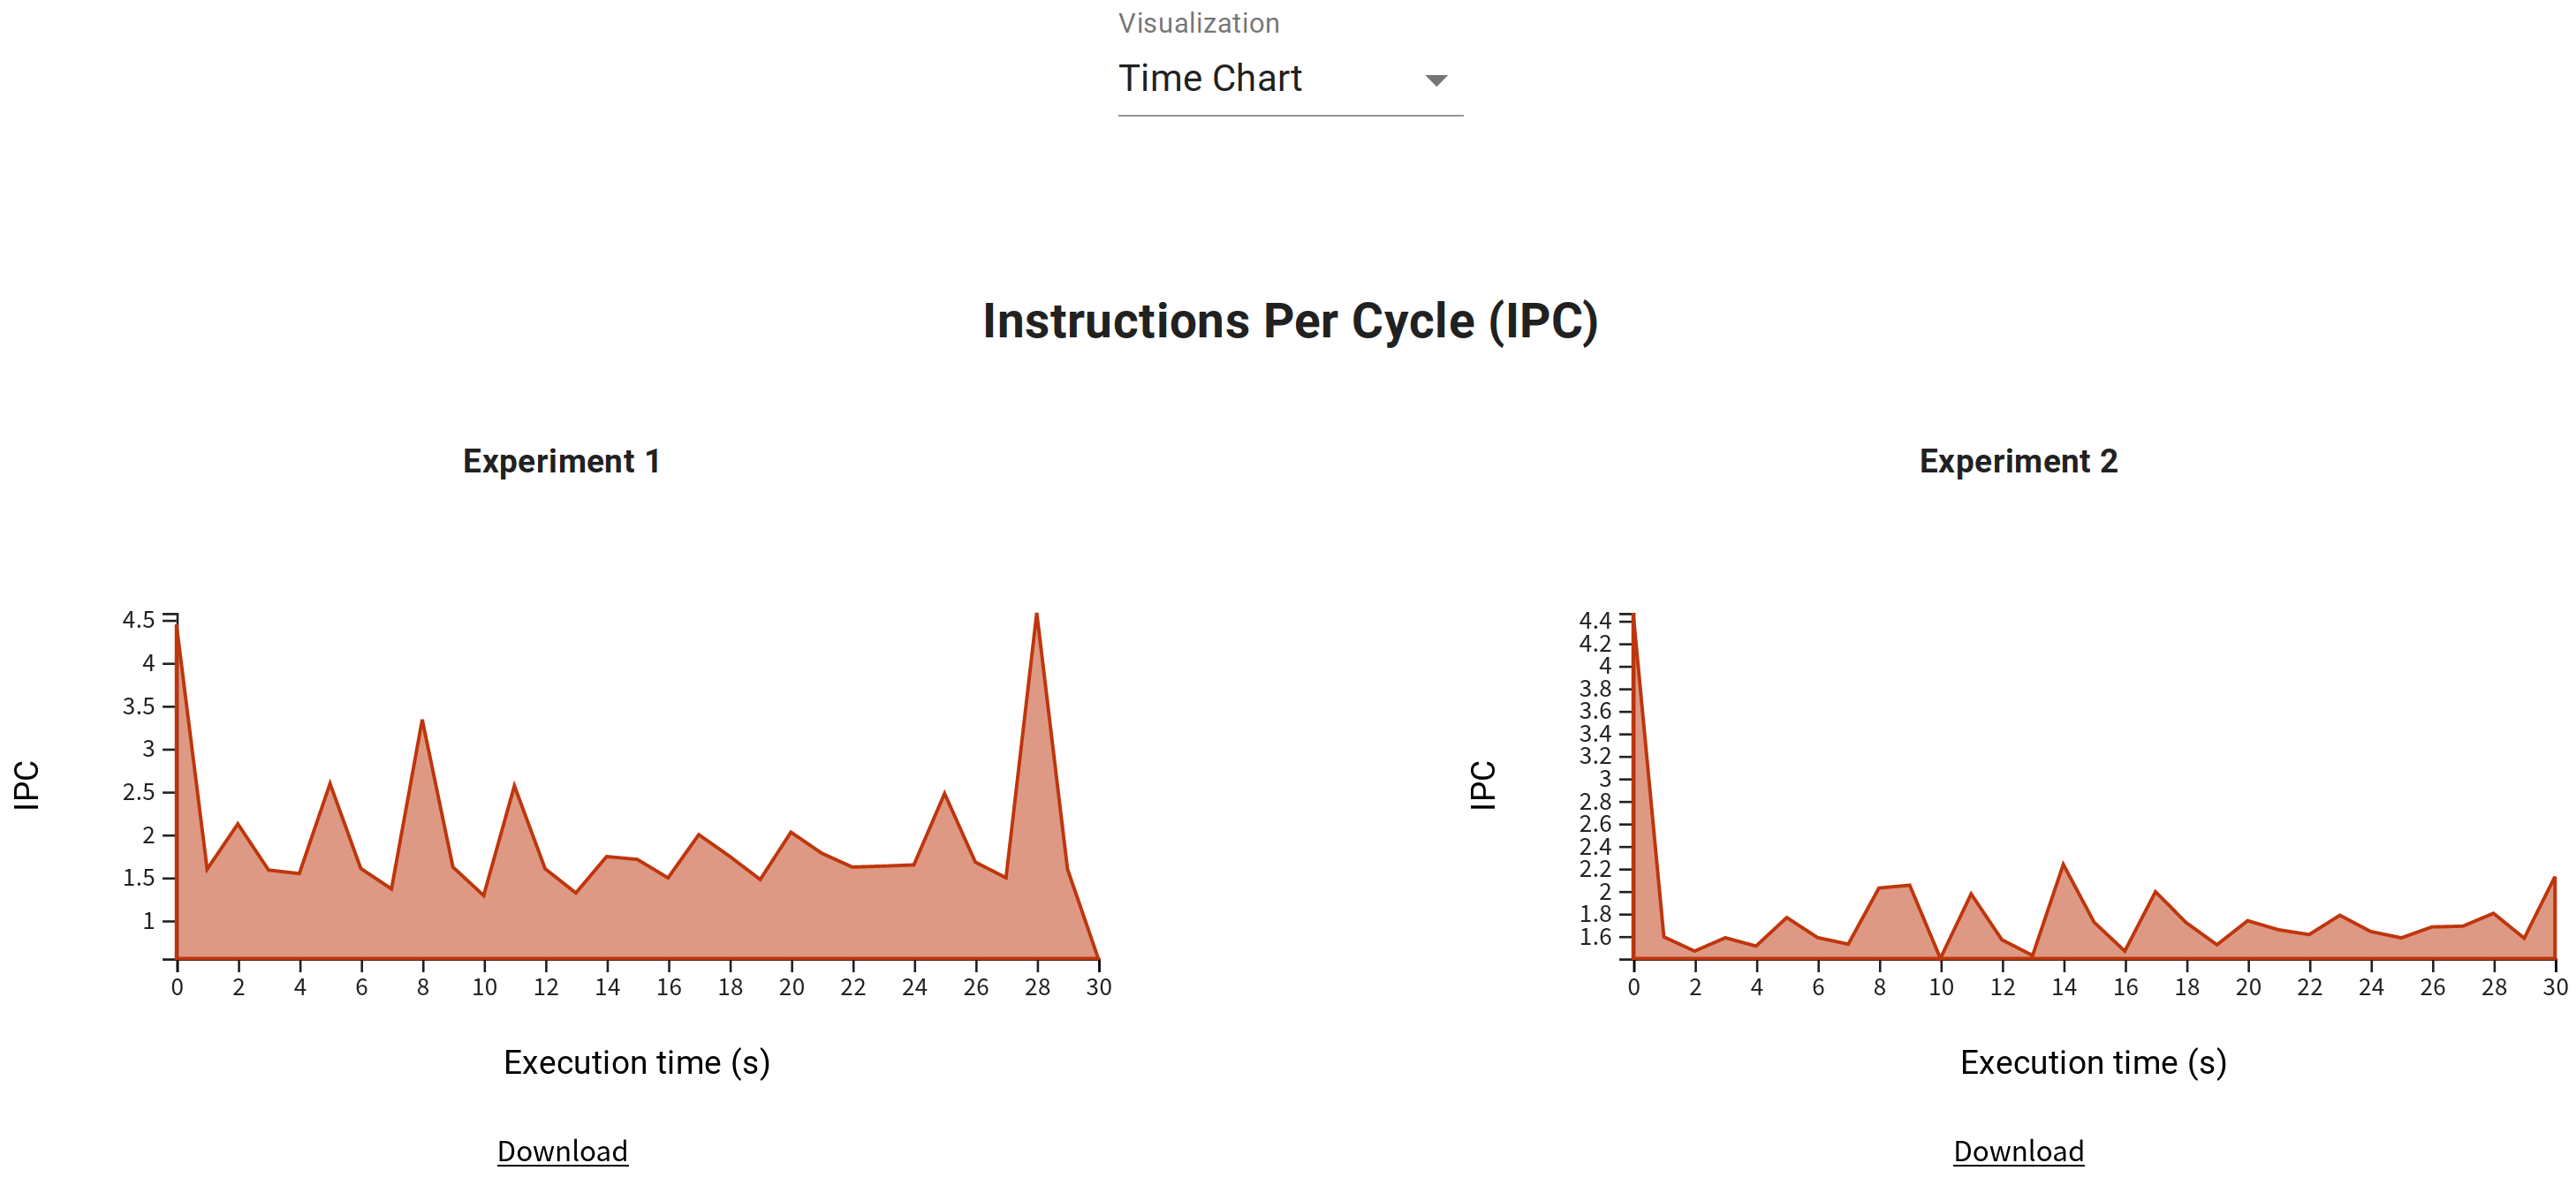
\includegraphics[width=1.0\columnwidth]{../pictures/visperf-section-3.png}
    \caption{VisPerf section ``Performance evaluation metrics''.}
    \label{figure:visperf-section-2}
\end{figure}
